\section{運用(坂本)}

運用は,東工大松永研の地上局(3.3節)を用いて運用した.コマンドのアップリンクは東工大からのみ行う設計である.一方,ダウンリンクについては,東工大地上局で受信を行うだけではなく,世界中のアマチュア無線家に受診協力していただいた.以下では東工大地上局の運用と,アマチュア無線家による受信協力に分けて記述する.

\subsection{東工大地上局での運用}

OrigamiSat-1の東工大上空の運用時間は,1日のうちにおおむね午前は8時ごろ,9時半ごろの2回と,午後は夜8時ごろと9時半ごろの2回であった.初期運用は地上実験を多く経験した熟練者によってのみ運用したが,次第に1回の運用につき2名の体制でシフトを組んで運用した.UHF/VHFの運用の手順については,地上局ソフトウェアを開発した飯島が詳細な運用手順書を作成したので,そちらを参考のこと.
\begin{itemize}
	\item OP-S1-0112  OrigamiGSC説明書
\end{itemize}

また,地上局は東工大松永研の施設を借用していたので,鍵の管理方法など,松永先生と施設使用の条件を取り決めて使用させてもらった.松永研の高価な通信機材を無断でOrigamiSat-1開発場所に持ち出していた前科があったため,そのようなことが二度とないよう丁寧な対応を試みた.
\begin{itemize}
	\item OP-S1-0113 松永研地上局使用ルール
	\item OP-S1-0107 松永研借用物品リスト
\end{itemize}

シフトの決定については,STKで可視時間を予測し,参加可能な時間を調整したうえでシフトを決定.シフトを失念しないよう,Slackで自動にリマインダを送る仕組みを活用した(当初,失念するメンバーが数人いたため,少しずつシステムを改善していった).
また,運用の日報については,Googleフォームに入力すると運用の履歴が残り,さらにその日報がSlackで全メンバーに共有されるようにした.
\begin{figure}[H]
	\centering
	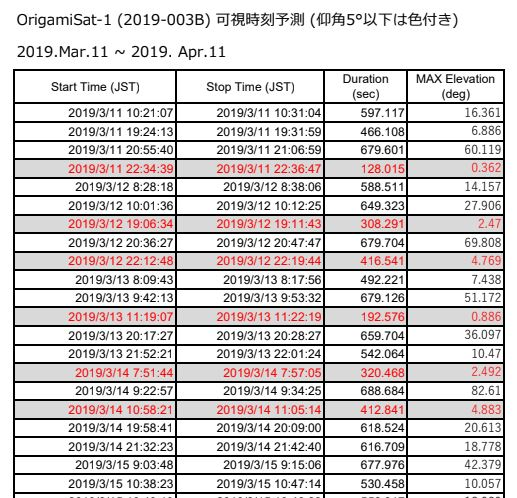
\includegraphics[width=.8\textwidth]{07/fig/7-1-1.jpg}
	\caption{可視時刻予測リストの例}
	\label{fig7-1-1}
\end{figure}
\begin{figure}[H]
	\centering
	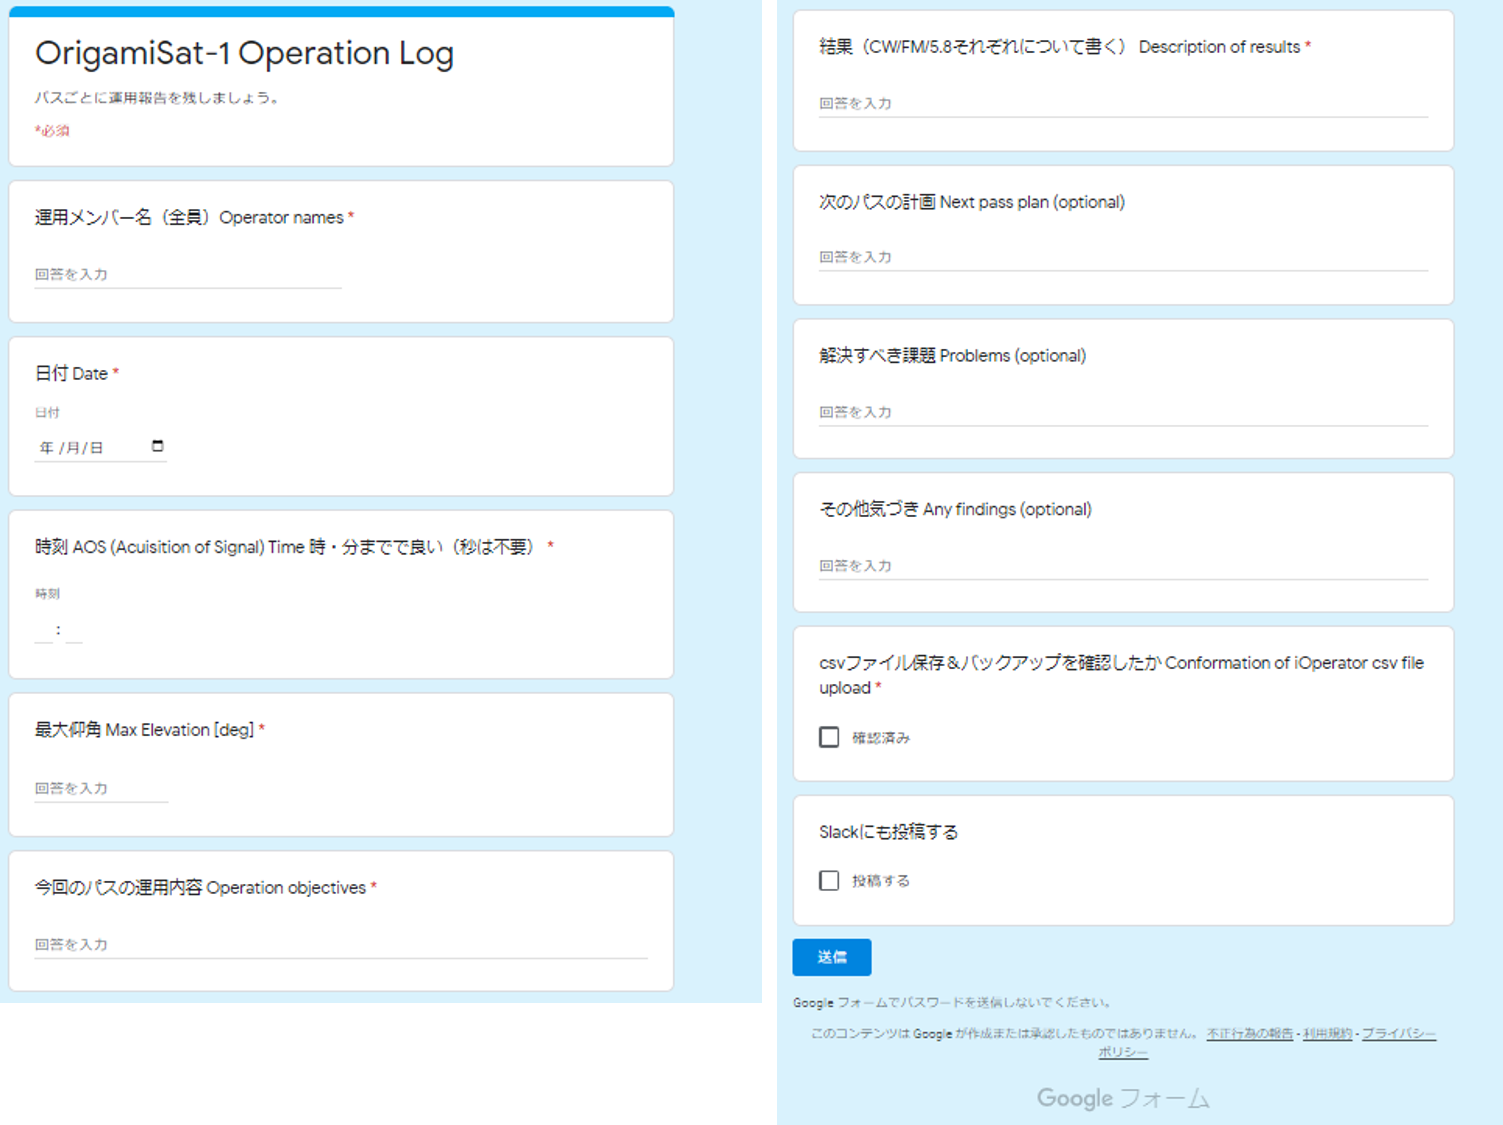
\includegraphics[width=.8\textwidth]{07/fig/7-1-2.png}
	\caption{Googleフォームによる運用記録入力}
	\label{fig7-1-2}
\end{figure}

\subsection{アマチュア無線家による受信報告}

\subsubsection{アマチュア無線家らのイベントへの参加}
アマチュア無線家との協調を目指し,衛星開発責任者の坂本とプロジェクトマネージャの中西は,下記のイベントに参加してきた.
\begin{itemize}
	\item 執筆中
\end{itemize}

\subsubsection{受信協力の呼びかけと反応}
HPでの情報公開

アマチュア無線家向けの受信報告フォーム

データ解析ソフト

Twitter

SatNOGs

\subsubsection{QSLカードの発行}

執筆中